\documentclass{article}

% Configurações Gerais ---------------------------------------------------------
\usepackage[brazil]{babel}
\usepackage[utf8]{inputenc}
\usepackage[T1]{fontenc}
\usepackage{sbc-template}
\usepackage{amsmath}
\usepackage{graphicx}

% Definição de Comandos --------------------------------------------------------
\newcommand{\n}[1]{\bar{#1}}

% Informações Pessoais ---------------------------------------------------------
\title{Somador Completo e Subtrador de 4 bits}
\author{Emanuel Zabka\inst{1} \and{} Wanderson Henrique Camargo Rosa\inst{1}}
\address{Eletrônica Digital I --- 2012/1\\
Centro de Ciências Exatas e Tecnológicas\\
Universidade do Vale do Rio dos Sinos --- UNISINOS
\email{\{emanuelzabka,wandersonwhcr\}@gmail.com}
}

% Corpo do Documento -----------------------------------------------------------
\begin{document}

% Título -----------------------------------------------------------------------
\maketitle{}

% Descrição --------------------------------------------------------------------
\section{Descrição}
\label{sec:descricao}

Este trabalho visa apresentar um módulo somador completo e subtrador de 4
\textit{bits} que possui uma chave para distinguir o tipo de cálculo aritmético
que está sendo utilizado naquele momento. Todas as etapas do desenvolvimento
serão apresentadas, incluindo as tabelas verdade geradas que estão descritas na
Seção \ref{sec:tabelas-verdade}. Com todas as variações encontradas, foram
construídos os Mapas de Karnaugh para representação da saída utilizando portas
lógicas e suas simplificações em expressões booleanas na Seção
\ref{sec:simplificacao}.

A estrutura dos circuitos lógicos gerados, explicados de forma modular onde cada
conjunto de estruturas necessárias será definido, são exibidos na Seção
\ref{sec:circuito-logico}. Com base nesta estrutura, criou-se uma lista de
materiais, declarando cada componente que será utilizado, adicionando um
orçamento, na Seção \ref{sec:lista-de-materiais}. Por fim, a conclusão do
trabalho é apresentada na Seção \ref{sec:conclusao} e declara as espectativas
futuras deste projeto.

% Tabelas Verdade --------------------------------------------------------------
\section{Tabelas Verdade}
\label{sec:tabelas-verdade}

As tabelas verdade apresentam todas as possibilidades que determinado problema
pode apresentar e suas soluções quando aquele estado está definido. Iniciando o
estudo de um somador básico utilizando 1 \textit{bit}, temos a seguinte análise
do problema.

\begin{equation*}
    \begin{array}[b]{r}
        0+0=0\\
        0+1=1\\
        1+0=1\\
        1+1=0
    \end{array}
\end{equation*}

Dadas duas entradas, o resultado da soma binária destes valores é apresentado no
lado direito da equação. Porém, quando executamos o cálculo $1+1$ o seu
resultado é $1$ e temos um valor $1$ de \textit{bit} adicional, chamado
\textit{carry out}. Para sua representação, precisamos trabalhar com dois
\textit{bits} na saída, o resultado da soma e o valor de \textit{carry out},
apresentados abaixo.

\begin{equation*}
    \begin{array}[b]{r}
        0+0=00\\
        0+1=01\\
        1+0=01\\
        1+1=10
    \end{array}
\end{equation*}

A equação acima é valida para somadores de somente 1 \textit{bit}. Estes
somadores podem ser conectados em série, efetuando a soma de conteúdos na
entrada com valores maiores de 1 \textit{bit}. O problema é que o valor de
\textit{carry out} do \textit{bit} menos significativo adjacente ao atual deve
ser considerada, pois influi no resultado se o valor é igual a $1$. Considerando
esta ligação em série, devemos utilizar o valor de \textit{carry in} no cálculo
da soma atual, possibilitando assim a propagação do valor em cálculos executados
em \textit{bits} menos significativos. Portanto, teremos a seguinte tabela
verdade.

\begin{equation*}
    \begin{array}{|c|c|c||c|c|}
        \hline C_i & A & B & S & C_o\\
        \hline 0 & 0 & 0 & 0 & 0\\
        \hline 0 & 0 & 1 & 1 & 0\\
        \hline 0 & 1 & 0 & 1 & 0\\
        \hline 0 & 1 & 1 & 0 & 1\\
        \hline 1 & 0 & 0 & 1 & 0\\
        \hline 1 & 0 & 1 & 0 & 1\\
        \hline 1 & 1 & 0 & 0 & 1\\
        \hline 1 & 1 & 1 & 1 & 1\\
        \hline
    \end{array}
\end{equation*}

Considerando que $C_i$ e $C_o$ são os valores representantes para
\textit{carry in} e \textit{carry out}, respectivamente, o resultado da soma
entre os valores de $A$ e $B$ são apresentados em $S$. Quando o valor $C_i$ está
definido como $0$, o resultado $S$ possui características de uma porta lógica
\texttt{XOR}; quando o valor deste mesmo elemento está definido como $1$, o
resultado possui características de uma porta \texttt{XNOR}.

% Simplificação ----------------------------------------------------------------
\section{Simplificação}
\label{sec:simplificacao}

Com base na tabela verdade apresentada, temos como construir dois Mapas de
Karnaugh com 3 variáveis, utilizando com entrada os valores $A$, $B$ e $C_i$,
gerando assim as saídas $S$ e $C_i$.

\begin{equation*}
    \begin{array}{cccccc}
        \hline S    &   & AB &    &    &   \\
        \hline      &   & 00 & 01 & 11 & 00\\
        \hline C_i  & 0 &  0 &  1 &  0 &  1\\
        \hline      & 1 &  1 &  0 &  1 &  0\\
        \hline
    \end{array}
\end{equation*}

\begin{equation*}
    \begin{array}{cccccc}
        \hline C_o  &   & AB &    &    &   \\
        \hline      &   & 00 & 01 & 11 & 00\\
        \hline C_i  & 0 &  0 &  0 &  1 &  0\\
        \hline      & 1 &  0 &  1 &  1 &  1\\
        \hline
    \end{array}
\end{equation*}

Unindo as informações adjacentes no Mapa de Karnaugh, é possível encontrar as
expressões booleanas representantes consideradas ótimas. Estas expressões foram
modificadas para que o seu resultado esteja um pouco mais amigável, buscando
demonstrar uma forma mais visível da análise descrita na Seção
\ref{sec:tabelas-verdade}, utilizando menos portas lógicas.

\begin{eqnarray*}
    S   &=& \n{A}\n{B}C_i + \n{A}B\n{C_i} + ABC_i + A\n{B}\n{C_i}\\
    S   &=& C_i(AB + \n{A}\n{B}) + \n{C_i}(A\n{B} + \n{A}B)\\
    C_o &=& AB + AC_i + BC_i\\
    C_o &=& AB + C_i(A + B)
\end{eqnarray*}

% Circuito Lógico --------------------------------------------------------------
\section{Circuito Lógico}
\label{sec:circuito-logico}

O circuito lógico para um somador binário simples pode ser construído utilizando
as seguintes portas lógicas, denotando as expressões booleanas encontradas
anteriormente.

\begin{figure}
    \centering{}
    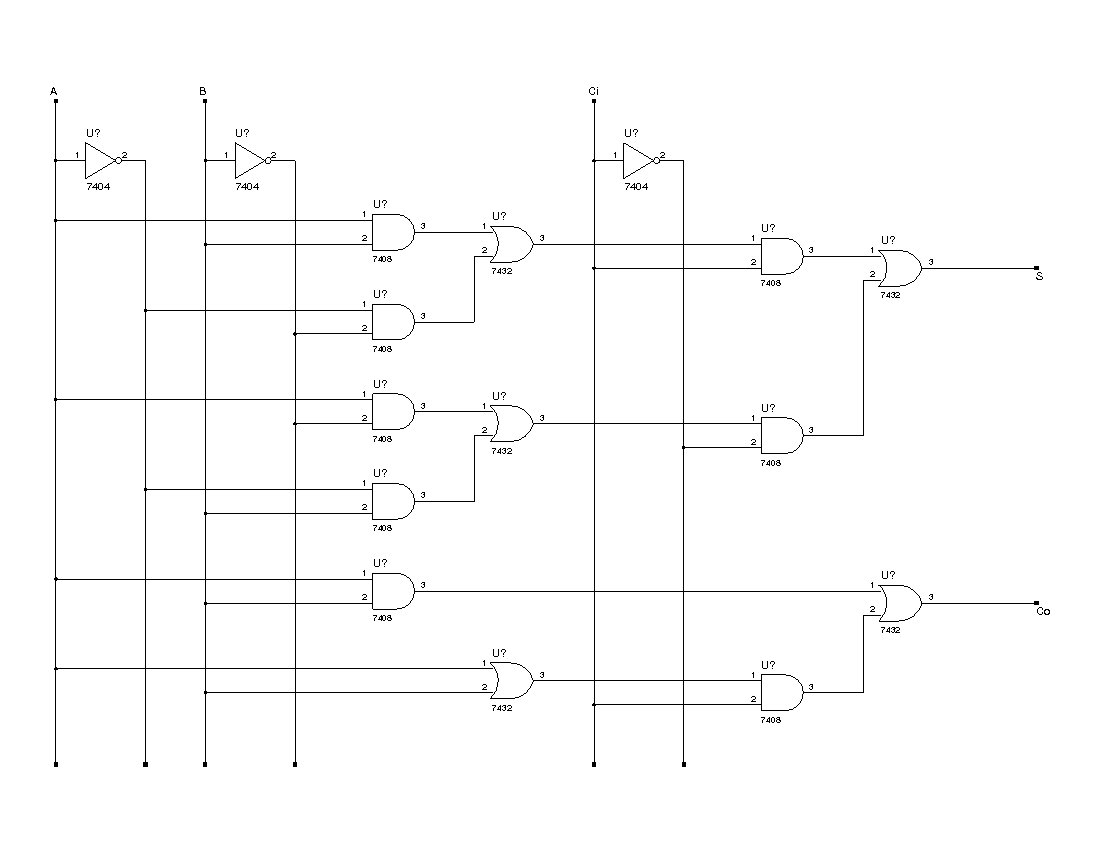
\includegraphics[width=\textwidth]{sources/ci1.jpg}
    \caption{Somador Binário}
    \label{fig:ci1}
\end{figure}

O somador apresentado na Figura \ref{fig:ci1} possui três entradas $A$, $B$ e
$C_i$ e possui saídas $S$ e $C_o$. Portanto, podemos representar a estrutura de
forma que abstraia a sua construção interna conforme Figura \ref{fig:sum}.

\begin{figure}
    \centering{}
    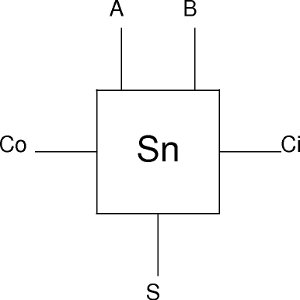
\includegraphics[scale=0.4]{sources/sum.jpg}
    \caption{Módulo Somador Binário}
    \label{fig:sum}
\end{figure}

Agora que temos o módulo básico somador de único \textit{bit}, podemos utilizar
o mesmo elemento e conectar muitos destes em série, criando um somador de 4
\textit{bits}.

% Somador de 4 bits ------------------------------------------------------------
\subsection{Somador de 4 bits}
\label{sec:somador-de-4-bits}

Um somador de 4 \textit{bits} é aquele que recebe como entrada dois valores
binários $A$ e $B$ de 4 casas e resulta numa saída de mesmo tamanho $S$.
Utilizando o componente criado anteriormente, podemos conectar 4 unidades em
série, onde a entrada $C_i$ de cada componente será conectada na saída $C_o$ do
componente em série. Os componentes na posição mais e menos significativa não
receberão conexão ainda.

\begin{figure}
    \centering{}
    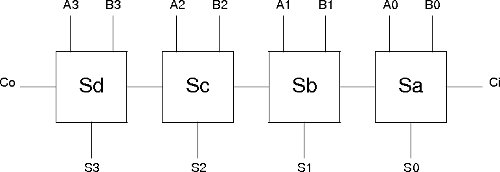
\includegraphics[scale=0.8]{sources/sums.jpg}
    \caption{Somador Binário de 4 bits}
    \label{fig:sums}
\end{figure}

Como especificamos este conjunto de elementos, podemos abstrair sua estrutura da
mesma forma que da aplicada às portas lógicas e definir um módulo somador de 4
\textit{bits} que possui 4 entradas para valores $A$ e para $B$, uma entrada
$C_i$ e uma saída $C_o$, bem como as 4 saídas resultado do somatório $S$.

\begin{figure}
    \centering{}
    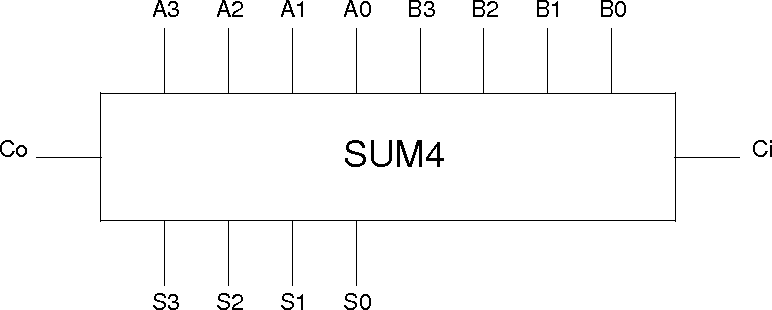
\includegraphics[scale=0.4]{sources/sum4.png}
    \caption{Módulo Somador Binário de 4 bits}
    \label{fig:sum4}
\end{figure}

% Lista de Materiais -----------------------------------------------------------
\section{Lista de Materiais}
\label{sec:lista-de-materiais}

% Subtrador de 4 bits ----------------------------------------------------------
\section{Subtrador de 4 bits}
\label{sec:subtrador-de-4-bits}

Possuindo um somador de 4 bits apresentado na Seção \ref{sec:somador-de-4-bits}
e definido conforme Figura \ref{fig:sum4}, podemos criar um módulo adicional que
inverte os valores de entrada de $B$ se o $C_i$ está em nível alto,
possibilitando assim a subtração.

Primeiramente, vamos especificar a tabela verdade para o problema, considerando
como valores de entrada $B$ e $C_i$ e como saída $B'$, criando um circuito
eletrônico para solucionar este problema.

\begin{equation*}
    \begin{array}{|c|c||c|}
        \hline B & C_i & B'\\
        \hline 0 & 0 & 0\\
        \hline 0 & 1 & 1\\
        \hline 1 & 0 & 1\\
        \hline 1 & 1 & 0\\
        \hline
    \end{array}
\end{equation*}

Podemos então verificar que temos uma definição de porta lógica \texttt{XOR} com
estes parâmetros. Temos então a expressão booleana da tabela verdade declarada.

\begin{eqnarray*}
    B' &=& B\n{C_i} + \n{B}C_i
\end{eqnarray*}

Utilizando a expressão booleana encontrada, vamos criar o circuito
correspontente para os valores.

\begin{figure}
    \centering{}
    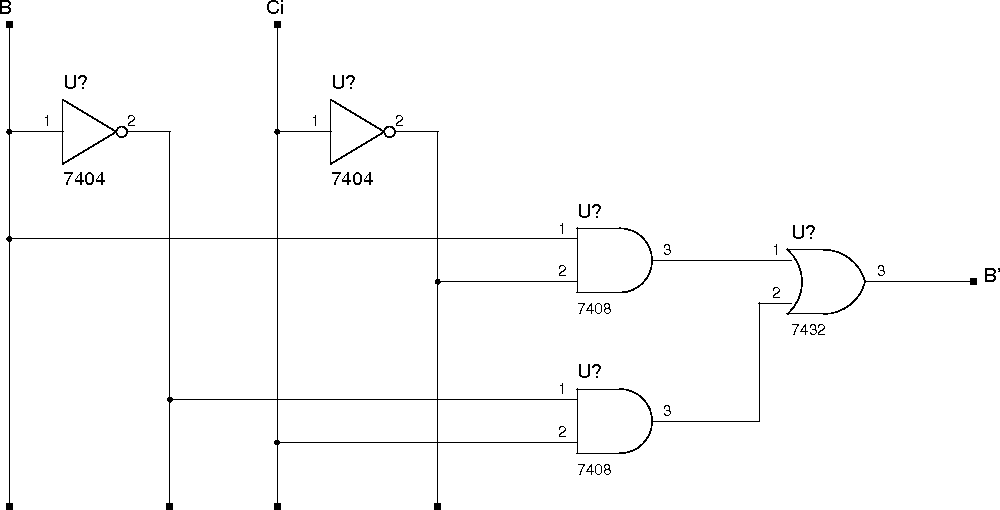
\includegraphics[scale=0.4]{sources/ci2.png}
    \caption{Inversor de Valores para B}
    \label{fig:ci2}
\end{figure}

O circuito correspondente pode ser generalizado num módulo único, possuindo duas
entradas $B$ e $C_i$ e uma saída $B'$ que inverte o sinal de $B$ se $C_i$ está
em nível alto.

\begin{figure}
    \centering{}
    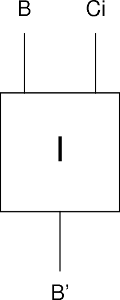
\includegraphics[scale=0.4]{sources/i.png}
    \caption{Módulo Inversor de 1 bit}
    \label{fig:i}
\end{figure}

O somador de 4 bits possui uma entrada $B$ de 4 casas, então podemos utilizar
este componente inversor 4 vezes, utilizando o mesmo sinal $C_i$ como entrada
nos 4 elementos.

\begin{figure}
    \centering{}
    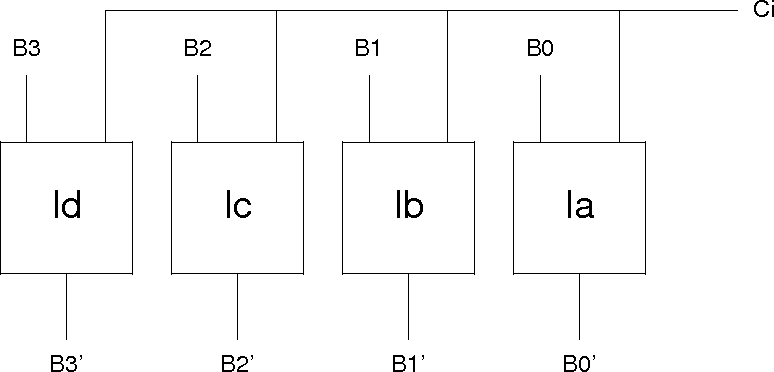
\includegraphics[scale=0.4]{sources/is.png}
    \caption{Utilização de 4 Módulos Inversores de 1 bit}
    \label{fig:is}
\end{figure}

Especificando esta estrutura, podemos criar uma estrutura abstrata que
representa um módulo inversor de 4 bits.

\begin{figure}
    \centering{}
    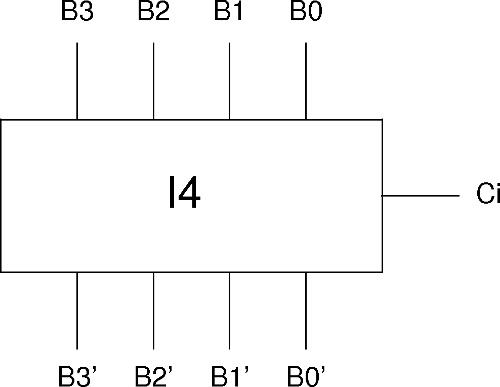
\includegraphics[scale=0.4]{sources/i4.png}
    \caption{Módulo Inversor de 4 bits}
    \label{fig:i4}
\end{figure}

Com este módulo desenvolvido, podemos anexá-lo ao somador de 4 bits. Quando o
valor de $C_i$ estiver em nível alto, os valores de $B$ serão invertidos,
executando assim uma subtração binária.

\begin{figure}
    \centering{}
    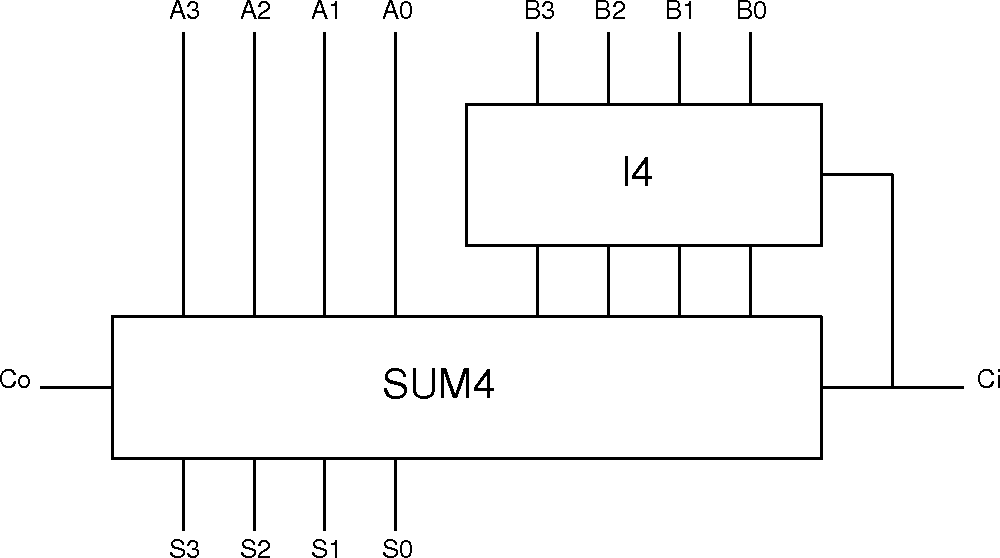
\includegraphics[scale=0.4]{sources/sumsub.png}
    \caption{Somador Completo de 4 bits com Subtrador}
    \label{fig:sumsub}
\end{figure}

% Conclusão --------------------------------------------------------------------
\section{Conclusão}
\label{sec:conclusao}

\end{document}
